\section{Framework pour la modélisation des SdSs}

\begin{frame}{Concepts et objectifs de la modélisation d'un SdS}

\begin{block}{Objectifs }
\begin{itemize}
\item Exactitude : modéliser les CSs, leurs ressources et objectifs
d'interaction
\item Précision : modéliser les décisions architecturales 
\end{itemize}
\end{block}

\begin{block}{Problématique}
La frontière des SdSs est floue. Il est difficile de savoir quelles
informations ont un impact sur le SdS.\\
\centering
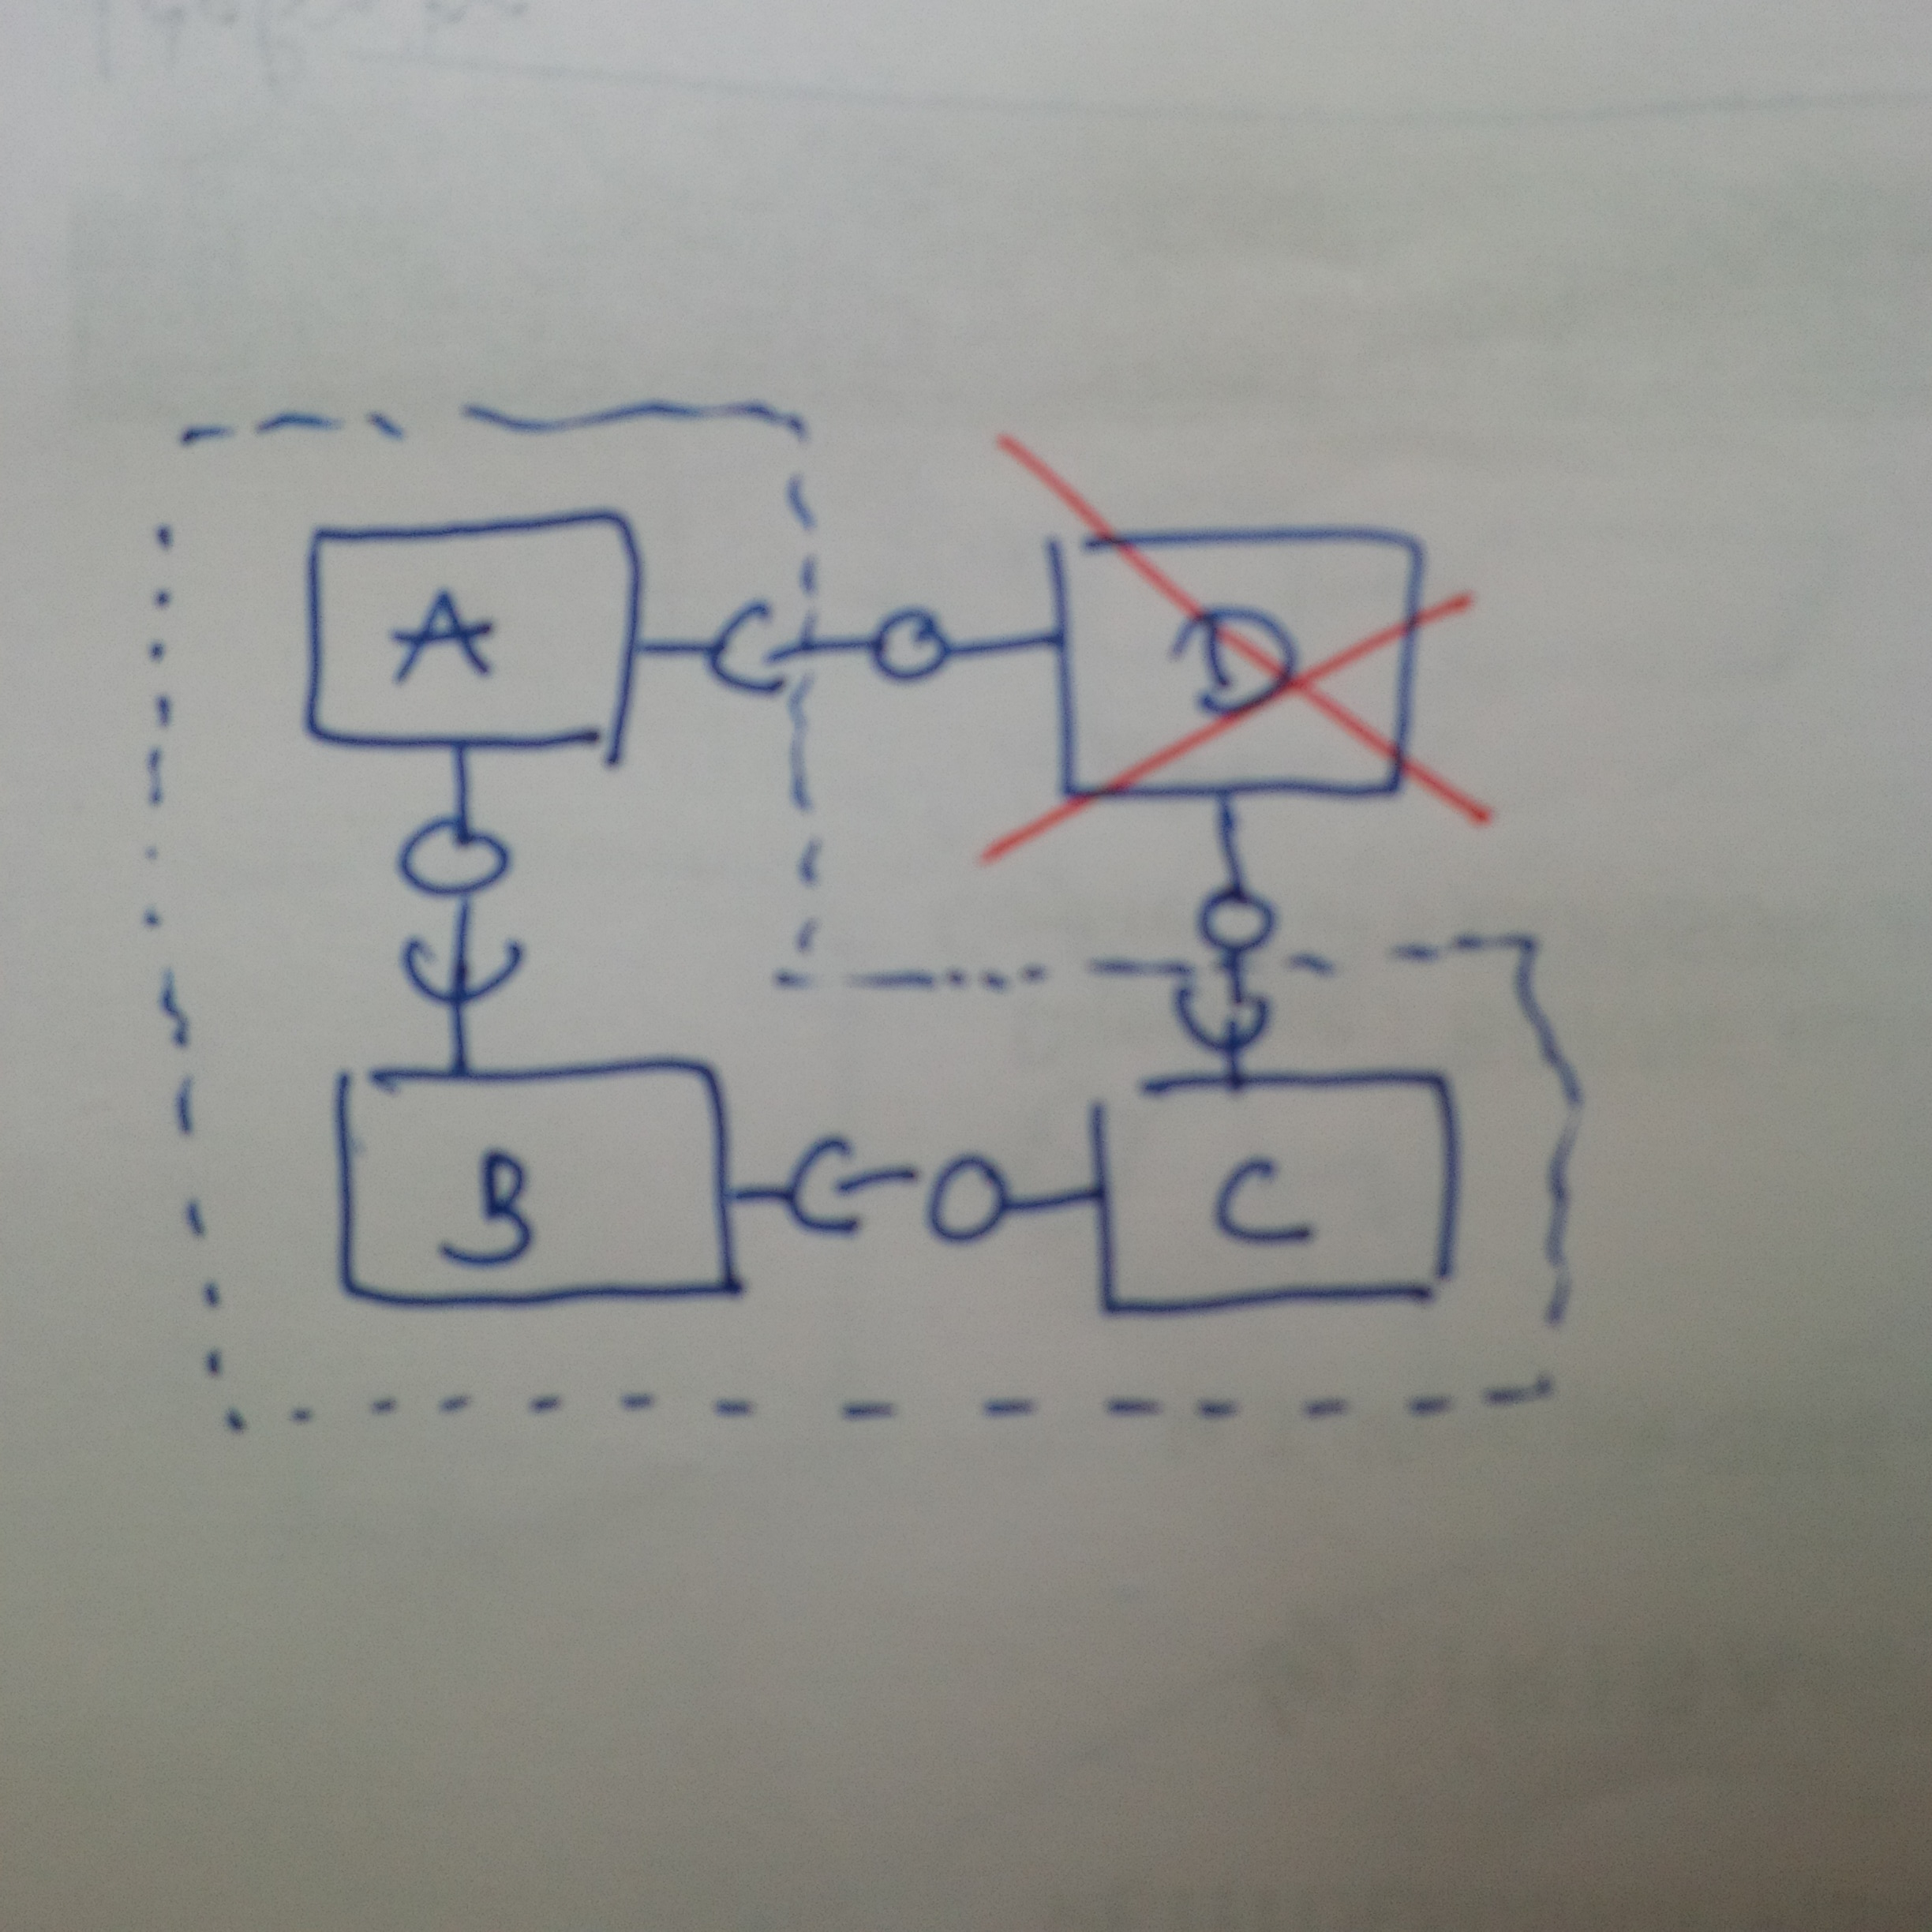
\includegraphics[scale=0.025]{imgs/slide_section1_probleme_frontiere.jpg}
\end{block}

\begin{block}{Approche}
\centering
Étude des langages et processus de modélisation.
\begin{figure} 
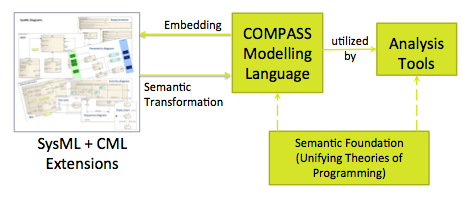
\includegraphics[width=4cm, height=1.5cm]{imgs/compass.png}
\hspace{0.5cm}
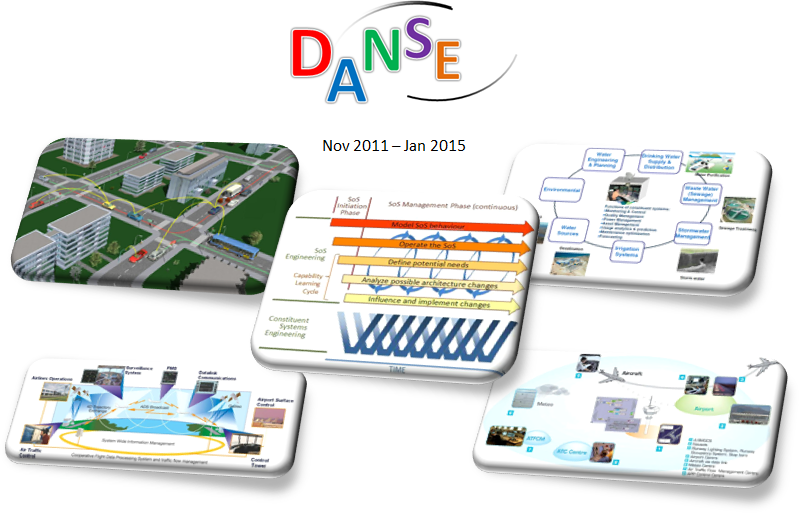
\includegraphics[width=4cm, height=1.5cm]{imgs/danse.png}
\end{figure}
\end{block} 

\end{frame}

\begin{frame}{SySML}
\begin{columns}
\begin{column}{0.5\textwidth}
Elements modélisés : 
\begin{itemize}
\item block
\item port
\item flux
\item allocation
\end{itemize}
\end{column}
\begin{column}{0.5\textwidth}
Diagrammes : 
\begin{itemize}
\item diagramme de block
\item diagramme de block interne
\item diagramme d'exigence
\item diagramme d'activité, d'état, etc.
\end{itemize}
\end{column}
\end{columns}
\begin{block}{Avantages et limite}
Avantages : 
\begin{itemize}
\item description connectivité
\item traçabilité
\item standardisation
\end{itemize}
Limite :
\begin{itemize}
\item absence de parti pris
\end{itemize}
\end{block}
\end{frame}

\begin{frame}{UPDM et utilisation par DANSE}
\end{frame}

%\begin{frame}{Comparaison de DANSE et COMPASS}
%- objectif de modélisation des vues pareil\\
%- utilisation des diagrammes différentes pour modéliser les objetctifs d'interaction\\
%les points négatifs : \\
%- pas de vérification de l'exactide. raffinement des propriétés dans des langages formelles\\
%\end{frame}

\begin{frame}{Stratégie de modélisation}
\end{frame}

\begin{frame}{Cas d'étude}
\begin{block}{Mission}
protection des
personnes, des biens et de l’environnement
\end{block}

\only<1>{
\begin{figure}
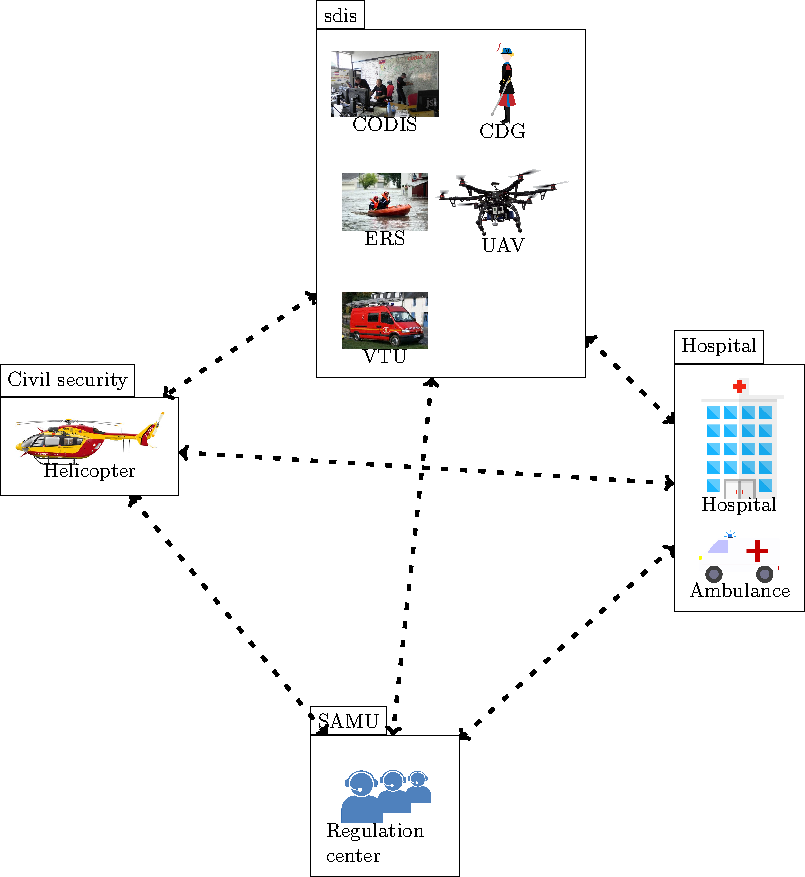
\includegraphics[width=0.5\textwidth, height=0.5\textwidth]{imgs/fig_sos_overview.pdf}
\end{figure}}

\only<2>{
\begin{figure}
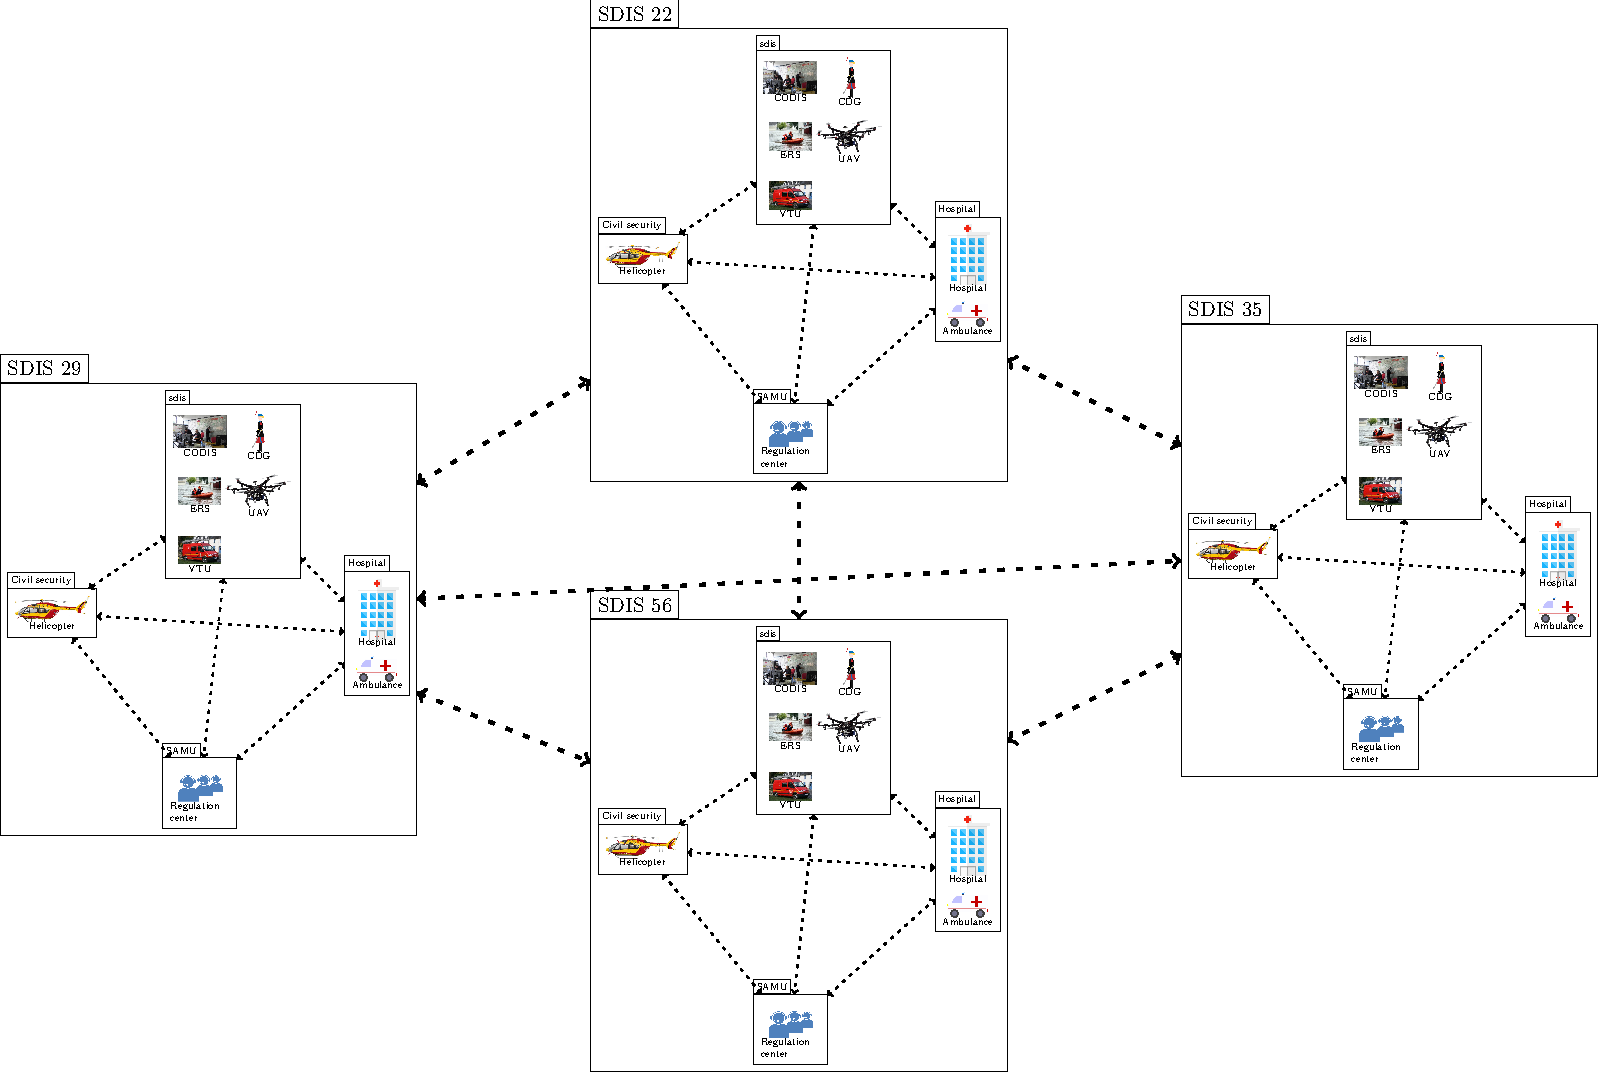
\includegraphics[width=0.5\textwidth, height=0.5\textwidth]{imgs/fig_sos_boundary.pdf}
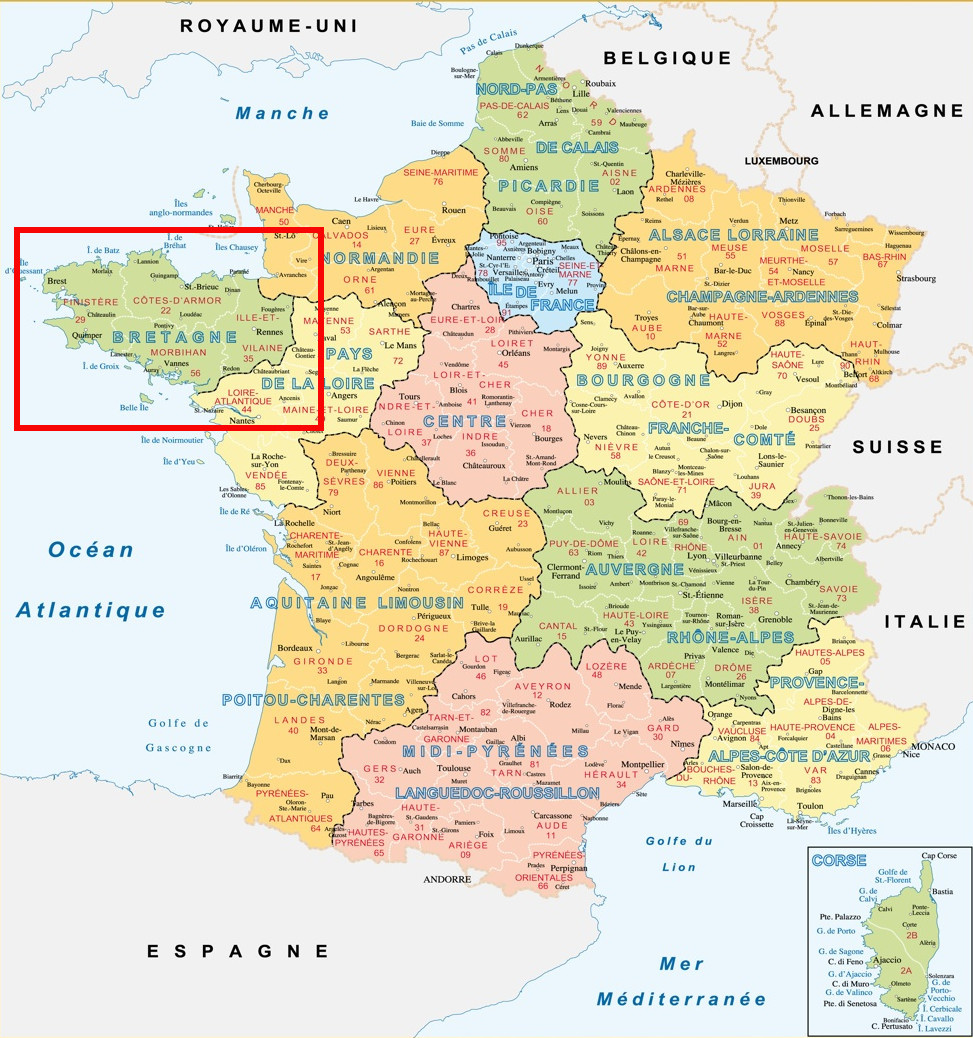
\includegraphics[scale=0.05]{imgs/carte_france_13_regions-2.jpg}
\end{figure}}

\only<3>{
chaine de commandement
}

\only<4>{
\begin{table}[]
\begin{tabular}{cc}
\multicolumn{2}{l}{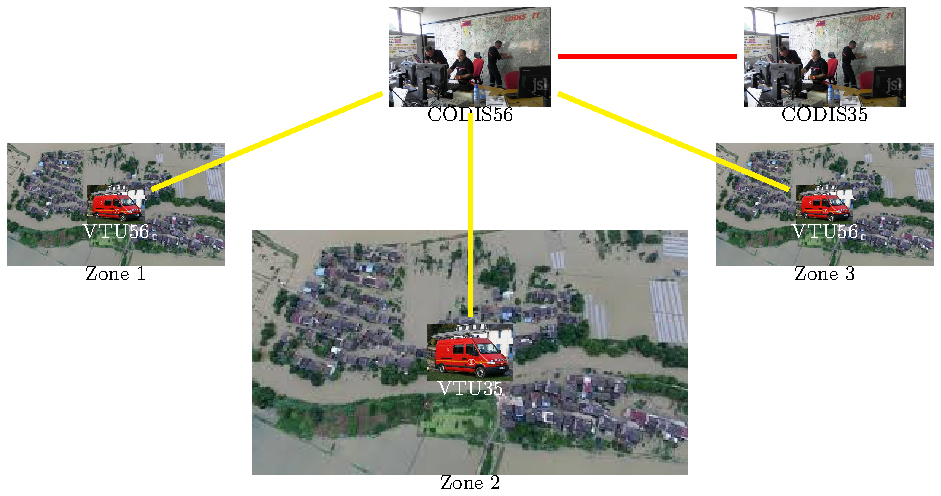
\includegraphics[scale=0.3]{imgs/fig_overview_conf1.pdf}}  \\
\multicolumn{2}{l}{Collaboration opérationnelle interdepartementale} \\
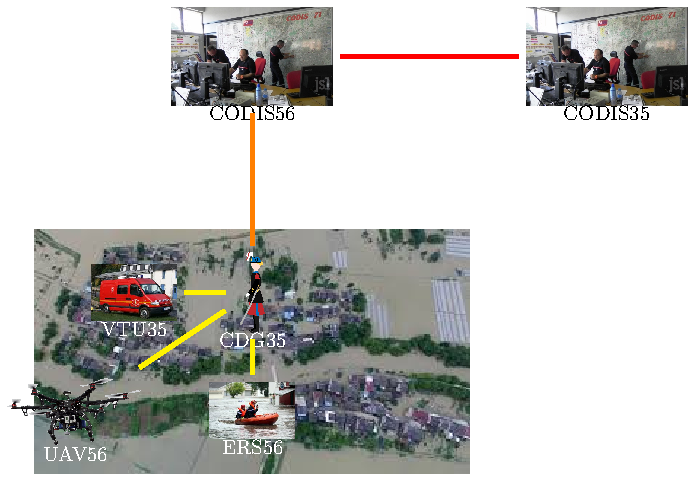
\includegraphics[scale=0.3]{imgs/fig_overview_conf2.pdf}            &
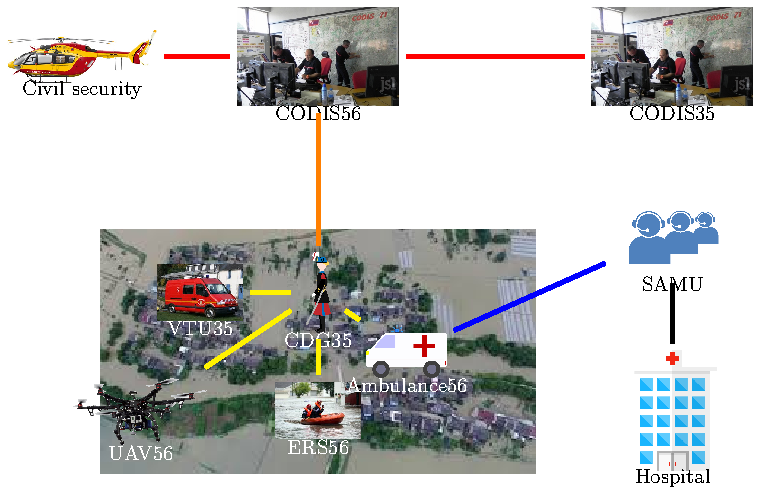
\includegraphics[scale=0.3]{imgs/fig_overview_conf3.pdf}          \\
Collaboration tactique et stratégique inter. dep.       &
Collaboration médicale    
\end{tabular}
\end{table}
}

\end{frame}

\begin{frame}{Modélisation}

\only<1>{
\begin{figure}
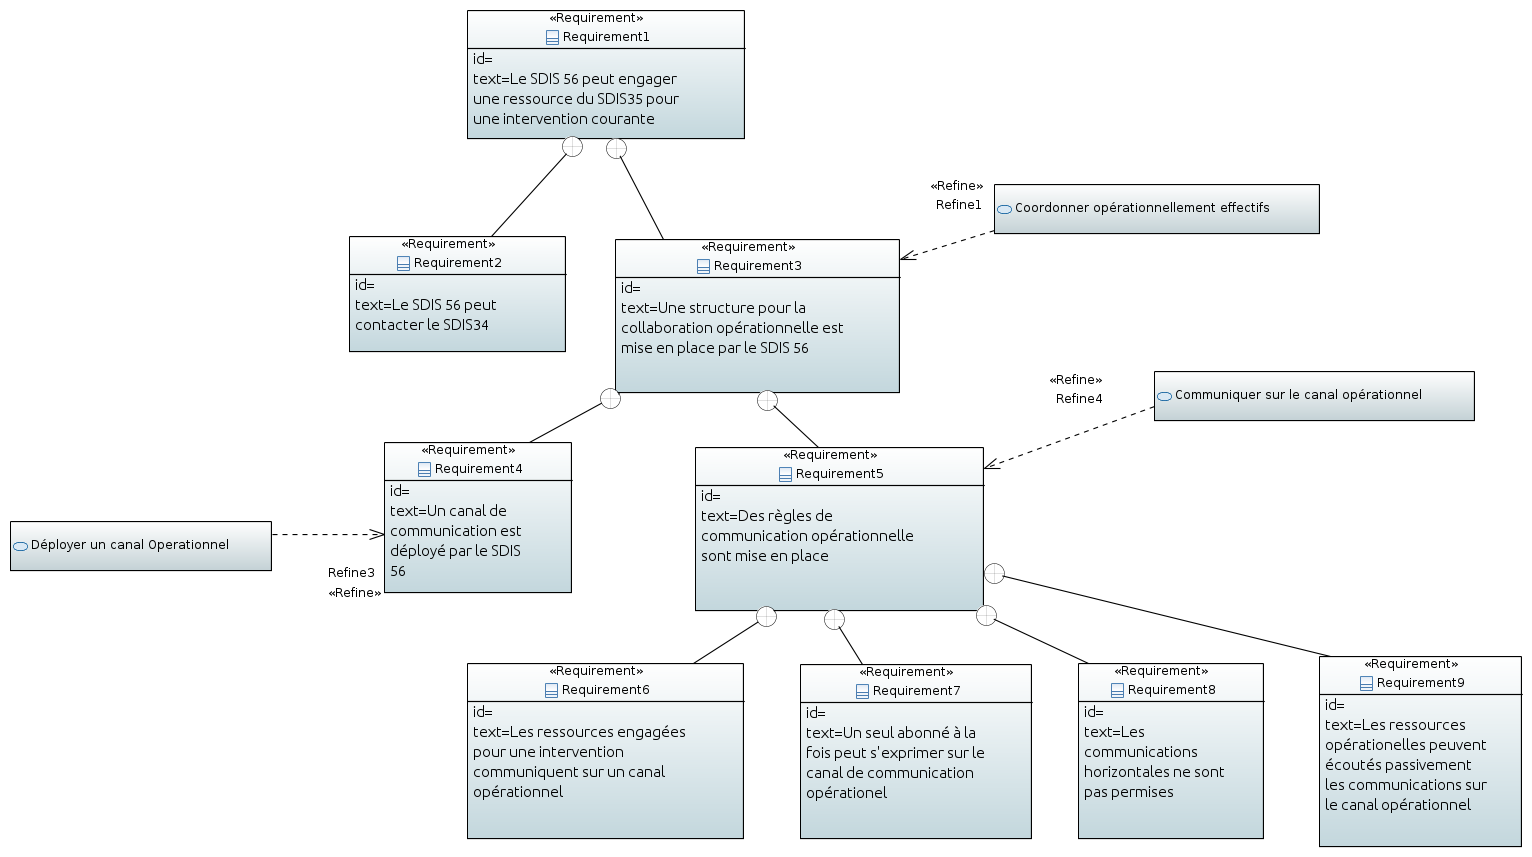
\includegraphics[width=0.5\textwidth, height=0.5\textwidth]{imgs/requirement_cas_1.PNG}
\end{figure}
}

\only<2>{
\begin{figure}
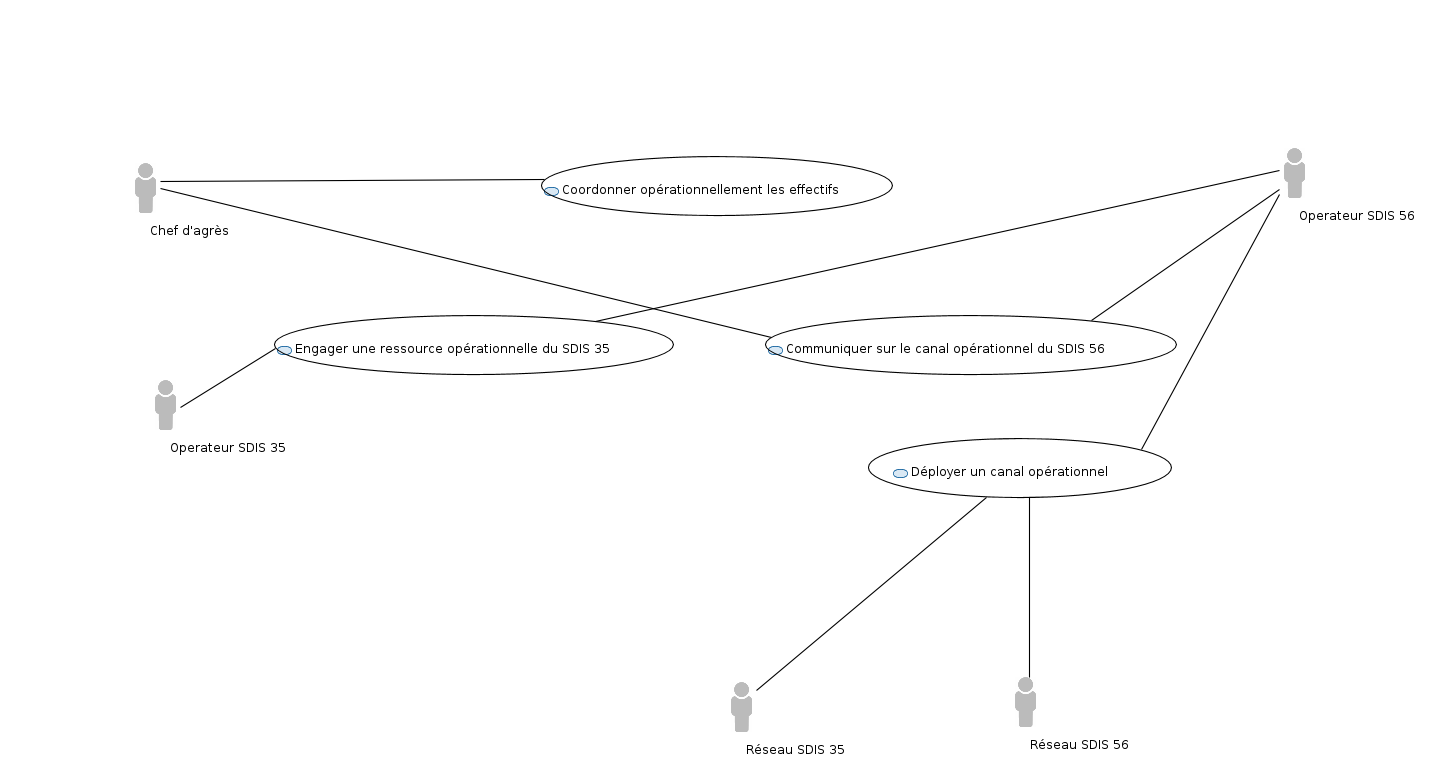
\includegraphics[width=0.5\textwidth, height=0.5\textwidth]{imgs/Collaboration_operationnelle_entre_le_SDIS_56_et_le_SDIS_35.PNG}
\end{figure}
}
\only<3>{
\begin{figure}
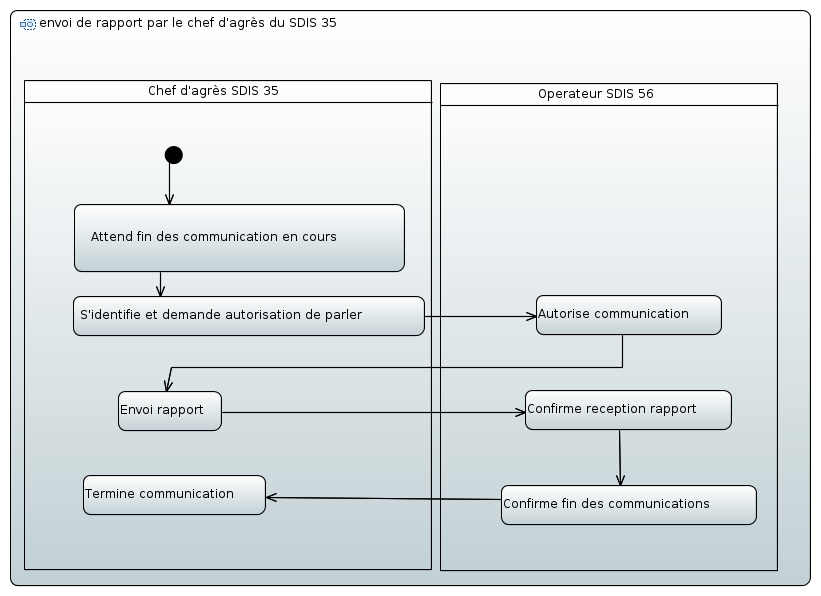
\includegraphics[width=0.5\textwidth, height=0.5\textwidth]{imgs/Reception_de_rapport.PNG}
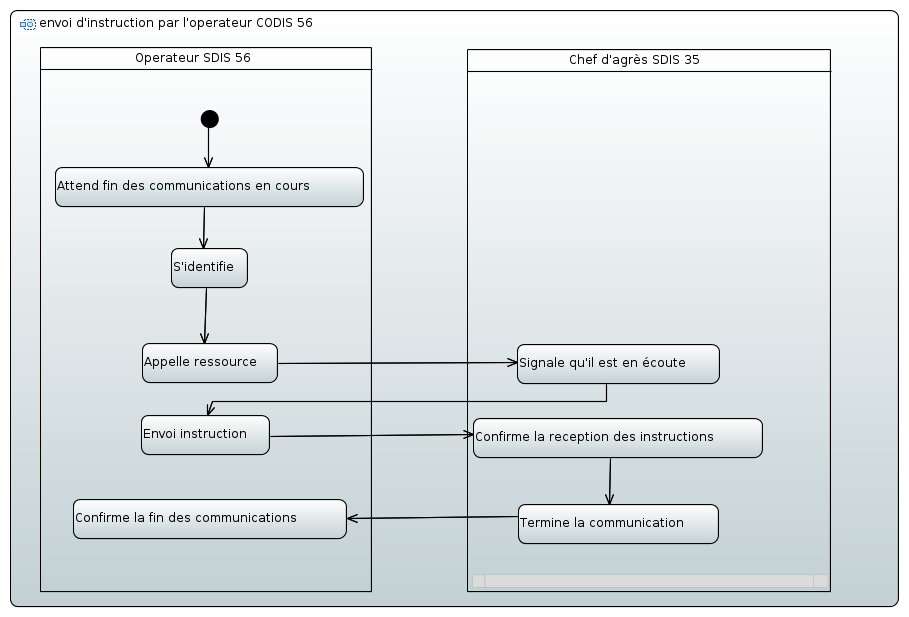
\includegraphics[width=0.5\textwidth, height=0.5\textwidth]{imgs/Envoie_de_rapport.PNG}
\end{figure}
}

\only<4>{
\begin{figure}
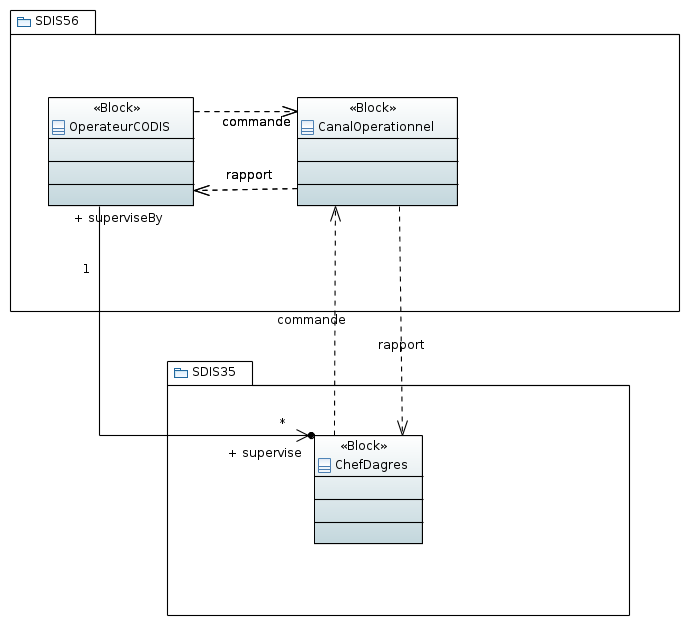
\includegraphics[width=0.5\textwidth, height=0.5\textwidth]{imgs/ov4-cas1.PNG}
\end{figure}
}

\only<5>{
\begin{figure}
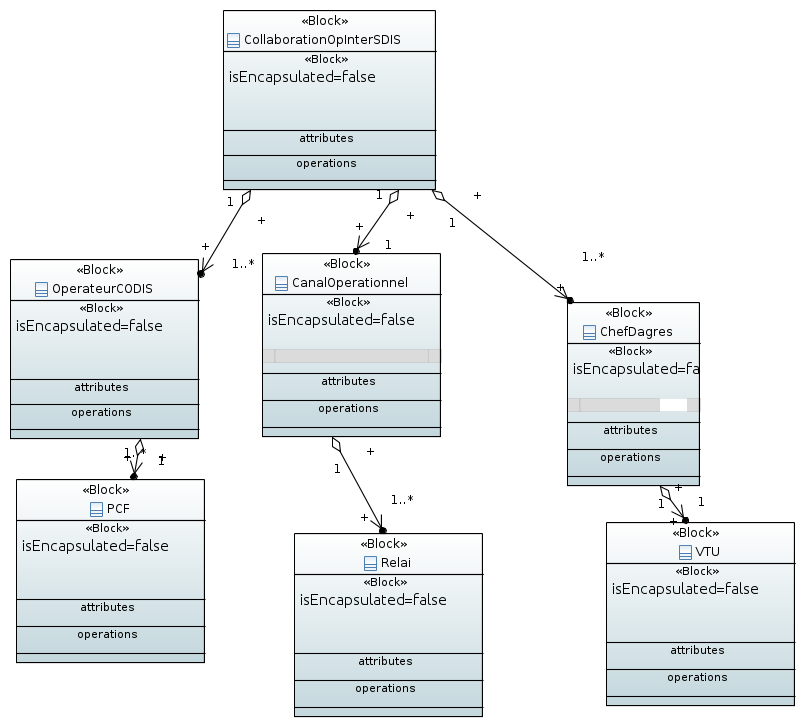
\includegraphics[width=0.5\textwidth, height=0.5\textwidth]{imgs/sv1-bdd-cas1.PNG}
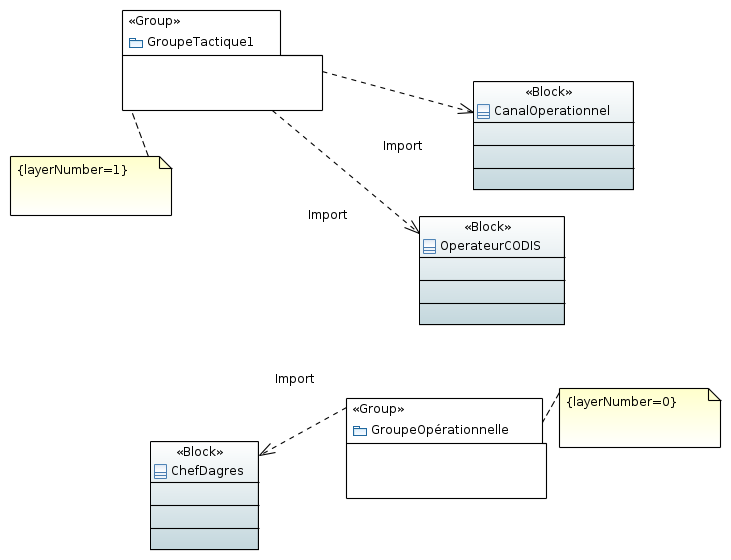
\includegraphics[width=0.5\textwidth, height=0.5\textwidth]{imgs/sv-1_package_conf1.PNG}
\end{figure}
}

\only<6>{
\begin{figure}
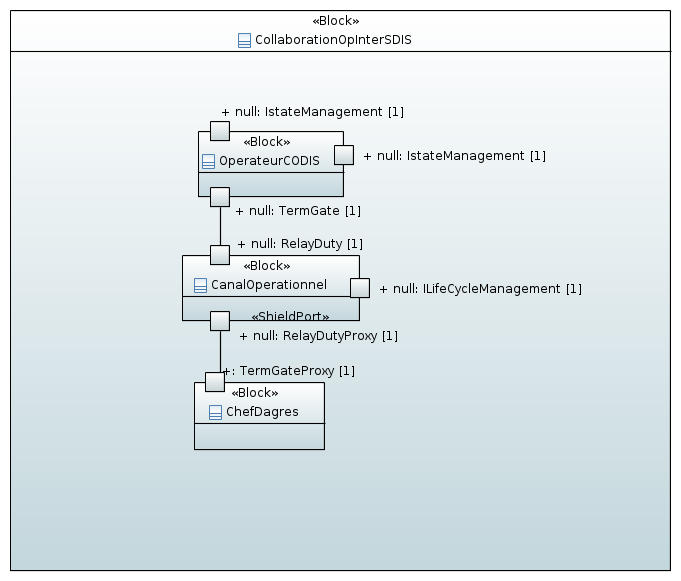
\includegraphics[width=0.5\textwidth,
height=0.5\textwidth]{imgs/sv1-bdi-cas1.PNG}
\end{figure}
}
\end{frame}

\begin{frame}{Résumé}
\end{frame}
